\usetikzlibrary{decorations.pathreplacing}
\usetikzlibrary{calc}
\tikzstyle{ydn}=[draw,minimum size=1em]
\tikzstyle{brace}=[thick, decoration={brace}, decorate]
\usetikzlibrary{decorations.shapes}
\tikzset{paint/.style={ draw=#1!50!black, fill=#1!50 }}
\tikzstyle{dots}=[decorate, 
         decoration={shape backgrounds, 
                     shape size=0.5mm, 
                     shape sep={0.5mm, between borders}},
         paint=black]
\usepackage{xparse}

%%%
%%
\newcommand{\ytThreeTwo}{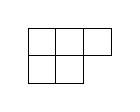
\begin{tikzpicture}[node distance=1em,auto]
  \node [ydn] (a) {};
  \node [ydn] (b) [right of=a] {};
  \node [ydn] (c) [right of=b] {};
  \node [ydn] (d) [below of=a] {};
  \node [ydn] (e) [below of=b] {};
\end{tikzpicture}}

  %%%%..%%
  %%
  %
% .
% .
  %
\DeclareDocumentCommand\ytTwoBoth{ m m g }{
\IfNoValueT {#3} {\def \posnum {0.5}}
\IfNoValueF {#3} {\def \posnum {#3}}
\begin{tikzpicture}[node distance=1em, auto]
  \node [ydn] (a) {};
  \node [ydn] (b) [right of=a] {};
  \node [ydn] (c) [right of=b] {};
  \node [minimum size=1em] (d) [right of=c] {};
  \draw [dots] ($ (d.west) + (0.8mm,0) $) -- ($ (d.east) + (-0.5mm,0) $);
  \node [ydn] (e) [right of=d] {};
  \node [ydn] (f) [below of=a] {};
  \node [ydn] (g) [below of=f] {};
  \node [minimum size=1em] (h) [below of=g] {};
  \draw [dots] ($ (h.north) + (0,-0.8mm) $) -- ($ (h.south) $);
  \node [ydn] (i) [below of=h] {};
  \node [ydn] (j) [below of=b] {};
  \draw [brace] ($ (a.north west) + (0,0.25em) $) -- ($ (e.north east) + (0,0.25em) $) node [pos=0.5] {\small $#1$};
  \draw [brace, decoration={mirror}] ($ (a.north west) + (-0.25em,0) $) -- ($ (i.south west) + (-0.25em,0) $) node [pos=\posnum, rotate=90, yshift=1em, xshift=-1.2em] {\small $#2$};
\end{tikzpicture}
}


  %%%...%%%
  %
% .
% .
  %
\newcommand{\ytWedgeStdRepn}[2]{
\begin{tikzpicture}[node distance=1em, auto]
  \node [ydn] (a) {};
  \node [ydn] (b) [right of=a] {};
  \node [ydn] (c) [right of=b] {};
  \node [minimum size=1em] (d) [right of=c] {};
  \draw [dots] ($ (d.west) + (0.8mm,0) $) -- ($ (d.east) + (-0.5mm,0) $);
  \node [ydn] (e) [right of=d] {};
  \node [ydn] (f) [below of=a] {};
  \node [ydn] (g) [below of=f] {};
  \node [minimum size=1em] (h) [below of=g] {};
  \draw [dots] ($ (h.north) + (0,-0.8mm) $) -- ($ (h.south) $);
  \node [ydn] (i) [below of=h] {};
%  \node [ydn] (j) [below of=b] {};
  \draw [brace] ($ (a.north west) + (0,0.25em) $) -- ($ (e.north east) + (0,0.25em) $) node [pos=0.5] {\small $#1$};
  \draw [brace, decoration={mirror}] ($ (a.north west) + (-0.25em,0) $) -- ($ (i.south west) + (-0.25em,0) $) node [pos=0.5, rotate=90, yshift=1em, xshift=-1.2em] {\small $#2$};
\end{tikzpicture}
}

%%%%
%%%
%
%
%
\newcommand{\ytFourThreeOneOneOne}{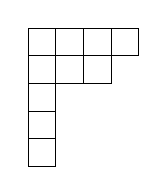
\begin{tikzpicture}[node distance=1em,auto]
  \node [ydn] (a1) {};
  \node [ydn] (a2) [right of=a1] {};
  \node [ydn] (a3) [right of=a2] {};
  \node [ydn] (a4) [right of=a3] {};
  \node [ydn] (b1) [below of=a1] {};
  \node [ydn] (b2) [below of=a2] {};
  \node [ydn] (b3) [below of=a3] {};
  \node [ydn] (c1) [below of=b1] {};
  \node [ydn] (d1) [below of=c1] {};
  \node [ydn] (e1) [below of=d1] {};
\end{tikzpicture}}

%%%...%%%
%
\newcommand{\ytStdRepn}[1]{
\begin{tikzpicture}[node distance=1em,auto]
  \node [ydn] (a) {};
  \node [ydn] (b) [right of=a] {};
  \node [ydn] (c) [right of=b] {};
  \node [minimum size=1em] (d) [right of=c] {};
  \draw [dots] ($ (d.west) + (0.8mm,0) $) -- ($ (d.east) + (-0.5mm,0) $);
  \node [ydn] (e) [right of=d] {};
  \node [ydn] (f) [below of=a] {};
  \draw [brace] ($ (a.north west) + (0,0.25em) $) -- ($ (e.north east) + (0,0.25em) $) node [pos=0.5] {\small $#1$};
\end{tikzpicture}
}

%%%...%%%
%
\newcommand{\ytAltStdRepn}[1]{\rotatebox{90}{
\begin{tikzpicture}[node distance=1em,auto]
  \node [ydn] (a) {};
  \node [ydn] (b) [right of=a] {};
  \node [ydn] (c) [right of=b] {};
  \node [minimum size=1em] (d) [right of=c] {};
  \draw [dots] ($ (d.west) + (0.8mm,0) $) -- ($ (d.east) + (-0.5mm,0) $);
  \node [ydn] (e) [right of=d] {};
  \node [ydn] (f) [below of=e] {};
  \draw [brace] ($ (a.north west) + (0,0.25em) $) -- ($ (e.north east) + (0,0.25em) $) node [pos=0.5] {\small $#1$};
\end{tikzpicture}
}}

%%%%...%%%
\newcommand{\ytTrivRepn}[1]{
\begin{tikzpicture}[node distance=1em,auto]
  \node [ydn] (a1) {};
  \node [ydn] (a2) [right of=a1] {};
  \node [ydn] (a3) [right of=a2] {};
  \node [minimum size=1em] (a4) [right of=a3] {};
  \draw [dots] ($ (a4.west) + (0.8mm,0) $) -- ($ (a4.east) + (-0.5mm,0) $);
  \node [ydn] (a5) [right of=a4] {};
  \draw [brace] ($ (a1.north west) + (0,0.25em) $) -- ($ (a5.north east) + (0,0.25em) $) node [pos=0.5] {\small $#1$};
\end{tikzpicture}
}

  %
  %
% .
% .
  %
\newcommand{\ytAltRepn}[1]{
\begin{tikzpicture}[node distance=1em,auto]
  \node [ydn] (a1) {};
  \node [ydn] (b1) [below of=a1] {};
  \node [ydn] (c1) [below of=b1] {};
  \node [minimum size=1em] (d1) [below of=c1] {};
  \draw [dots] ($ (d1.north) + (0,-0.5mm) $) -- ($ (d1.south) + (0,0.8mm) $);
  \node [ydn] (e1) [below of=d1] {};
  \draw [brace,decoration=mirror] 
      ($ (a1.north west) + (-0.25em,0) $) -- 
      ($ (e1.south west) + (-0.25em,0) $) 
      node [pos=0.5, rotate=90, yshift=1em, xshift=-0.5em] 
      {\small $#1$};
\end{tikzpicture}
}

  %%%
  %%
% .
% .
  %
\DeclareDocumentCommand\ytThreeTwoN{ m g }{
\IfNoValueT {#2} {\def \posnum {0.5}}
\IfNoValueF {#2} {\def \posnum {#2}}
\begin{tikzpicture}[node distance=1em,auto]
  \node [ydn] (a1) {};
  \node [ydn] (a2) [right of=a1] {};
  \node [ydn] (a3) [right of=a2] {};
  \node [ydn] (b1) [below of=a1] {};
  \node [ydn] (b2) [right of=b1] {};
  \node [ydn] (c1) [below of=b1] {};
  \node [minimum size=1em] (d1) [below of=c1] {};
  \draw [dots] ($ (d1.north) + (0,-0.5mm) $) -- ($ (d1.south) + (0,0.8mm) $);
  \node [ydn] (e1) [below of=d1] {};
  \draw [brace,decoration=mirror] 
      ($ (a1.north west) + (-0.25em,0) $) -- 
      ($ (e1.south west) + (-0.25em,0) $) 
      node [pos=\posnum, rotate=90, yshift=1em, xshift=-0.5em] 
      {\small $#1$};
\end{tikzpicture}
}

  %%
  %%
  %%
  %  
% .
% .
  %
\newcommand{\ytTwoTwoTwoN}[1]{
\begin{tikzpicture}[node distance=1em,auto]
  \node [ydn] (a1) {};
  \node [ydn] (a2) [right of=a1] {};
  \node [ydn] (b1) [below of=a1] {};
  \node [ydn] (b2) [right of=b1] {};
  \node [ydn] (c1) [below of=b1] {};
  \node [ydn] (c2) [right of=c1] {};
  \node [ydn] (d1) [below of=c1] {};
  \node [minimum size=1em] (e1) [below of=d1] {};
  \draw [dots] ($ (e1.north) + (0,-0.5mm) $) -- ($ (e1.south) + (0,0.8mm) $);
  \node [ydn] (f1) [below of=e1] {};
  \draw [brace,decoration=mirror] 
      ($ (a1.north west) + (-0.25em,0) $) -- 
      ($ (f1.south west) + (-0.25em,0) $) 
      node [pos=0.5, rotate=90, yshift=1em, xshift=-0.5em] 
      {\small $#1$};
\end{tikzpicture}
}

  %%
  %%
% .
% .
  %
\DeclareDocumentCommand\ytTwoTwoN{ m g }{
\IfNoValueT {#2} {\def \posnum {0.5}}
\IfNoValueF {#2} {\def \posnum {#2}}
%\newcommand{\ytTwoTwoN}[1]{
\begin{tikzpicture}[node distance=1em,auto]
  \node [ydn] (a1) {};
  \node [ydn] (a2) [right of=a1] {};
  \node [ydn] (b1) [below of=a1] {};
  \node [ydn] (b2) [right of=b1] {};
  \node [ydn] (c1) [below of=b1] {};
  \node [minimum size=1em] (d1) [below of=c1] {};
  \draw [dots] ($ (d1.north) + (0,-0.5mm) $) -- ($ (d1.south) + (0,0.8mm) $);
  \node [ydn] (e1) [below of=d1] {};
  \draw [brace,decoration=mirror] 
      ($ (a1.north west) + (-0.25em,0) $) -- 
      ($ (e1.south west) + (-0.25em,0) $) 
      node [pos=\posnum, rotate=90, yshift=1em, xshift=-0.5em] 
      {\small $#1$};
\end{tikzpicture}
}


%%%%....%%
%%
\newcommand{\ytNTwo}[1]{
\begin{tikzpicture}[node distance=1em,auto]
  \node [ydn] (a1) {};
  \node [ydn] (a2) [right of=a1] {};
  \node [ydn] (a3) [right of=a2] {};
  \node [minimum size=1em] (a4) [right of=a3] {};
  \draw [dots] ($ (a4.west) + (0.8mm,0) $) -- ($ (a4.east) + (-0.5mm,0) $);
  \node [ydn] (a5) [right of=a4] {};
  \draw [brace] ($ (a1.north west) + (0,0.25em) $) -- ($ (a5.north east) + (0,0.25em) $) node [pos=0.5] {\small $#1$};
  \node [ydn] (b1) [below of=a1] {};
  \node [ydn] (b2) [below of=a2] {};
\end{tikzpicture}
}


%%%%....%%
%%
%
\newcommand{\ytNTwoOne}[1]{
\begin{tikzpicture}[node distance=1em,auto]
  \node [ydn] (a1) {};
  \node [ydn] (a2) [right of=a1] {};
  \node [ydn] (a3) [right of=a2] {};
  \node [minimum size=1em] (a4) [right of=a3] {};
  \draw [dots] ($ (a4.west) + (0.8mm,0) $) -- ($ (a4.east) + (-0.5mm,0) $);
  \node [ydn] (a5) [right of=a4] {};
  \draw [brace] ($ (a1.north west) + (0,0.25em) $) -- ($ (a5.north east) + (0,0.25em) $) node [pos=0.5] {\small $#1$};
  \node [ydn] (b1) [below of=a1] {};
  \node [ydn] (b2) [below of=a2] {};
  \node [ydn] (c1) [below of=b1] {};
\end{tikzpicture}
}
